\section[Metrology of the gradient magnetic field]
{Accuracy bound for gradient field estimation with atomic ensembles}
\thiswatermark{\put(1,-282){\color{l-grey}\rule{84pt}{88pt}}
\put(84,-282){\color{grey}\rule{410pt}{88pt}}}

\label{sec:gm}

\quotes{Ronald Fisher}{To consult the statistician after an experiment is finished is often merely to ask him to conduct a post mortem examination. He can perhaps say what the experiment died of.}

\lettrine[lines=2, findent=3pt, nindent=0pt]{I}{n} this chapter, one of the most fundamental two-parameter estimation tasks in magnetometry is considered, namely gradient magnetometry.
We will add the gradient of the magnetic field as the second parameter beside the constant (homogeneous) part of the field.
While most works in magnetometry with a single ensemble focus only on the determination of the strength and direction of the magnetic field, certain measurement schemes for the gradient have already been proposed and tested experimentally.
We study gradient magnetometry with an ensemble of atoms described by a very general probability distribution function for the position of the atoms, and considering atoms with an arbitrary spin.
Some schemes use an imaging of the ensemble with a high spatial resolution, however, they do not count as single-ensemble methods in the sense we use this expression in our paper, since in this case not only collective observables are measured  \cite{Vengalattore2007,Zhou2010,Koschorreck2011}.
There is a method based on collective measurements of the spin length of a fully polarized ensemble \cite{Behbood2013}.
Finally, there is a scheme where they use as a trial state a many-body singlet states, which is described in Ref.~\cite{Urizar-Lanz2013}.

We calculate precision bounds for estimating the gradient of the magnetic field based on the quantum Fisher information.
For quantum states that are invariant under the homogeneous magnetic field, a single parameter estimation is sufficient.
In contrast to this, for states that are sensitive to the homogeneous fields, a two-parameter estimation problem must be solved to obtain the gradient parameter, since the homogeneous field must also be taken into account.
We use our method to calculate precision bounds for gradient estimation with a chain of atoms and even with two spatially separated atomic ensembles which feel different magnetic fields.
As we said, we also consider a single atomic ensemble with an arbitrary density profile, in which atoms cannot be addressed individually, which is a very relevant case for experiments.
Our model can take into account even correlations between particle positions.

The atoms will be distributed along the $x$-axis, so $y=z=0$, and in principle they will be able to feel differences in the magnetic field at different points of the axis.
The magnetic field at the atoms will be given by a linear function of the position $x$
\begin{equation}
\bs{B}(x,0,0)=\bs{B}_0 +x \bs{B}_1 + O(x^2),
\end{equation}
where we will neglect the terms of order two or higher.
We will consider the magnetic field pointing along the $z$-direction direction only, $\bs{B}_0=B_0 \bs{k}$ and $\bs{B}_1=B_1\bs{k}$, where $\bs{k}$ is the unitary vector pointing on the $z$-direction.
For this configuration, due to the Maxwell equations, with no currents or changing electric fields, we have
\begin{align}
\nabla \cdotp \bs{B}&=0, \nonumber \\
\nabla \times \bs{B}&=\bs{0},
\end{align}
where $\bs{0}\equiv (0,0,0)$ is the 3-dimensional null vector.
This implies $\sum_{l=x,y,z} \partial_l B_l=0$ and $ \partial_m B_l - \partial_l B_m =0$ for all $l\ne m$, where $\partial_m\equiv \partial/\partial_m$ stands for the partial derivative over the variable $m$.
Thus, the spatial derivatives of the field components are not independent of each other.
However, in the case of a linear arranged particle ensemble only the derivative along the $x$-axis has an influence on the quantum dynamics of the atoms.

We will determine the precision bounds for the estimation of the magnetic field gradient $B_1$ based on the quantum Fisher information \cite{Paris2009,Braunstein1994,Holevo1982,Helstrom1976,Petz2002,Petz2008}.
In this context the Heisenberg and shot-noise scaling are defined as usual.
The achievable precision in terms of the number of particles scales as $\varinv{\theta}\sim N$ and $\varinv{\theta}\sim N^2$ for shot-noise scaling and Heisenberg scaling respectively.
We will show that with spin chains or two ensembles at different positions the Heisenberg scaling is possible.
Concerning the case of a single ensemble, we will show the following.
Since in such systems the atoms cannot be be individually addressed, we will assume that the quantum state is permutationally invariant.
We will show that for states insensitive to the homogeneous magnetic field, one can reduce the problem to a one-parameter estimation scenario.
Such states can arise in a single-ensemble scheme, however, it will be shown that the Heisenberg limit cannot be reached in this case.
When the state is sensitive to the homogeneous field, the spatial correlation between the atoms must be taken into account in order to show whether the system can overcome the shot-noise scaling and achieve the Heisenberg scaling.
Nevertheless, single-ensemble measurements have certain advantages since the spatial resolution can be higher and the experimental requirements are smaller since only a single ensemble must be prepared.

On the other hand, for states sensitive to the homogeneous field, the classical limit can be overcome only if the particle positions are highly correlated with each other.
Our calculations are generally valid for any measurement, thus they are relevant to many recent experiments \cite{Wasilewski2010,Eckert2006,Wildermuth2006, Wolfgramm2010,Koschorreck2011,Vengalattore2007,Zhou2010,Behbood2013}.
We note that in the case of the singlet, our precision bounds are saturated by the metrological scheme presented in Ref.~\cite{Urizar-Lanz2013}.

We can also connect our results to entanglement theory \cite{Werner1989,Horodecki2009,Guehne2009}.
We find that even in the case of gradient magnetometry the shot-noise scaling cannot be surpassed with separable states, while the Heisenberg scaling can be reached with entangled states.
However, in the single-ensemble scenario, the shot-noise scaling can be surpassed only if the particle positions are correlated, which is the case if the particles attract each other.
We will go into the details in Section~\ref{sec:gm-single-cloud}.

The chapter is organized as follows. In Section~\ref{sec:gm-the-setup}, we will present the setup of the system.
In Section~\ref{sec:gm-cramer-rao-bounds}, the metrological basic concepts used in the chapter are presented.
In Section~\ref{sec:gm-io-chain-and-two-ensembles}, we will show the results for the chain of ions and for when two distant ensembles are considered
In Section~\ref{sec:gm-single-cloud}, we restrict our calculations to single permutationally invariant atomic ensembles and we develop some particular cases, such as the singlet spin state or the totally polarized state.

\subsection{The setup}
\label{sec:gm-the-setup}

In this section, we will present the characteristics of our setup.
For simplicity, as well as following  recent experiments (e.g., Ref.~\cite{Koschorreck2011}), we will consider an ensemble of spin-$j$ particles placed in a one-dimensional trap or a chain.
Furthermore, we will assume that the particles are point-like and distinguishable.
On the other hand, we assume that the particles have a spin, which is a quantum degree of freedom.
Such a model is used typically to describe experiments with cold atomic ensembles.

Based on these considerations, we assume that the state is factorizable into a spatial and a spin part as
\be
\label{eq:gm-separated-internal-and-external}
\rho=\rho^{(\text{x})}\otimes\rho^{(\text{s})},
\ee
and that the spatial part can be characterized as an incoherent mixture of point-like particles that can be written as
\be
  \rho^{(\text{x})}=\int \prob(\bs{x}) \ketbra{\varphi_{\bs{x}}}{\varphi_{\bs{x}}}\,\text{d}^N\bs{x}.
  \label{eq:gm-pre-thermal-state}
\ee
where $\ket{\varphi_{\bs{x}}}$ is a pure state of each particle been placed at $\bs{x}=(x_1,x_2,\dots,x_N)$, respectively.
Each part of the state acts on different Hilbert spaces denoted by $\mathcal{H}^{(\text{x})}$ and $\mathcal{H}^{(\text{s})}$, respectively.
Note that we skip to write the superscript $(\text{x})$, denoting the Hilbert space to which $\ket{\varphi_{\bs{x}}}$ belongs, for simplicity.

In order to write the operators, including the state $\rho^{(\text{x})}$, acting on the Hilbert space $\mathcal{H}^{(\text{x})}$, we will invoke the completeness relation found in the literature \citep{Sakurai2010, Cohen-Tannoudji1977} for the spatial continuous Hilbert space
\be
  \int \ketbra{\bs{x}}{\bs{x}}\,\text{d}^N\bs{x} = \mtxid,
\ee
where $\ket{\bs{x}}=\ket{x_1}^{(1,\text{x})}\otimes\ket{x_2}^{(2,\text{x})}\cdots\otimes\ket{x_N}^{(N,\text{x})}$ is the tensor product of the position eigenvectors of each particle which obey
\be
  \braket{\bs{x}}{\bs{y}} = \delta(\bs{x}-\bs{y}),
\ee
where $\delta(\bs{x}-\bs{y})$ is the Dirac delta found in the literature \citep{Sakurai2010, Cohen-Tannoudji1977}.

To see how our notation works, let us write the vector of the position operators for each particle as $\hat{\bs{x}}\equiv(x^{(1)},x^{(2)},\dots,x^{(N)})$, where we used the $\hat{\cdot}$ notation on top of $\bs{x}$ to distinguish it from the vector of position variables.
It is known that $\hat{\bs{x}}$ acting on $\ket{\bs{x}}$ will give $\bs{x}\ket{\bs{x}}$ \cite{Sakurai2010, Cohen-Tannoudji1977}.
Hence,
\be
  \hat{\bs{x}} = \hat{\bs{x}}\mtxid = \hat{\bs{x}} \int \ketbra{\bs{x}}{\bs{x}}\,\text{d}^N\bs{x} = \int \hat{\bs{x}} \ketbra{\bs{x}}{\bs{x}}\,\text{d}^N\bs{x} = \int \bs{x} \ketbra{\bs{x}}{\bs{x}}\,\text{d}^N\bs{x}.
\ee
We can follow similar arguments to rewrite the pure state $\ket{\varphi_{\bs{x}}}$.
First, note also that the expectation value of the position operator for such a state is always $\bs{x}$.
Hence, such a state must be proportional to $\ket{\bs{x}}$.
On the other hand, a pure state must be normalized to one, hence, we can construct such a state by dividing the eigenvector $\ket{\bs{x}}$ by the square-root of its norm as
\be
  \ket{\varphi_{\bs{x}}} \equiv \frac{\ket{\bs{x}}}{\sqrt{\braket{\bs{x}}{\bs{x}}}}.
\ee
For illustrative purposes, we compute in this basis the expectation value of the position operator for these pure states as
\be
  \expect{\hat{\bs{x}}}_{\varphi_{\bs{x}}} = \braopket{\varphi_{\bs{x}}}{\int \bs{y} \ketbra{\bs{y}}{\bs{y}}\,\text{d}^N\bs{y}}{\varphi_{\bs{x}}} =
  \int \bs{y}
  \frac{\braket{\bs{x}}{\bs{y}}\braket{\bs{y}}{\bs{x}}}
  {\braket{\bs{x}}{\bs{x}}} \,\text{d}^N\bs{y} =
  \bs{x}\frac{\braket{\bs{x}}{\bs{x}}}{\braket{\bs{x}}{\bs{x}}} =
  \bs{x},
\ee
where in the step before the last we have used $\braket{\bs{y}}{\bs{x}}=\delta(\bs{y}-\bs{x})$ to compute the integral.
Using that $\braket{\bs{x}}{\bs{x}}=\delta(\bs{0})$, where $\bs{0}$ is a $N$-dimensional vector of zeros, we can rewrite the spatial state Eq.~\eqref{eq:gm-pre-thermal-state} as
\be
  \rho^{(\text{x})}=\int \frac{\prob(\bs{x})}{\delta(\bs{0})} \ketbra{\bs{x}}{\bs{x}}\,\text{d}^N\bs{x}.
  \label{eq:gm-thermal-state}
\ee
Note also that if the eigen-decomposition of the internal state is $\rho^{(\text{s})} = \sum_{\lambda} p_{\lambda}\ketbra{\lambda}{\lambda}$, then the whole state is decomposed as
\be
  \rho = \int\sum_{\lambda} \frac{\prob(\bs{x})}{\delta(\bs{0})} p_\lambda \ketbra{\bs{x},\lambda}{\bs{x},\lambda}\,\text{d}^N\bs{x},
  \label{eq:gm-eigendecomposition-of-state}
\ee
where $\ket{\bs{x},\lambda}$ is a shorthand for $\ket{\bs{x}}^{(\text{x})}\otimes\ket{\lambda}^{(\text{s})}$, the eigenstates, where their corresponding eigenvalues are in this case $\frac{\prob(\bs{x})}{\delta(\bs{0})} p_\lambda$.

At this point, we want to emphasize that our method could easily be extended to the case of Bose-Einstein condensates, or any other spatial configuration, not considered in this paper. In the case of BECs, the spatial state of the particles would be a pure state, and we would have $\rho^{(\text{x})}=(\ketbra{\Psi}{\Psi})^{\otimes N},$ where $\ket{\Psi}$ is a spatial single-particle state.

Although in our case the parameter to be estimated is $B_1$,
the time-evolution of the state is usually also affected by the second unknown parameter, the homogeneous field $B_0$, which means that we generally have to consider a two-parameter estimation problem.
The angular momentum of an individual atom is coupled to the magnetic field, yielding the following interaction term
\be
  h^{(n)}=\gamma B_z^{(n,\text{x})} \otimes j_z^{(n,\text{s})},
  \label{eq:gm-single-particle-hamiltonian}
\ee
where the operator $B_z^{(n)}=B_0+B_1 x^{(n)}$ acts on the spatial part of the $n^{\text{th}}$ particle Hilbert space $\mathcal{H}^{(n,\text{x})}$.

The sum  of all single-particle interactions with the magnetic field provide the total Hamiltonian
\be
\label{eq:gm-Htot}
H = \gamma \sum_{n=1}^N B_z^{(n,\text{x})} \otimes j_z^{(n,\text{s})},
\ee
which will generate the time evolution of the system.

We will calculate lower bounds on the precision of estimating $B_1$ based on measurements on the state after it passed through the unitary dynamics $U=\exp(-i\frac{H}{\hbar}t)$, where $t$ is the time spent by the system under the influence of the magnetic field.
The unitary operator can be rewritten in the following way
\be
\label{eq:gm-whole-unitary-b_i-encoded}
U=e^{-i \lpar b_0 H_0 + b_1 H_1 \rpar},
\ee
where the $b_i=\gamma B_i t/\hbar$ and therefore $b_1$ encodes the gradient of the magnetic field $B_1$.
Here, the generator describing the effect of the homogeneous field is  given as
\be
\label{eq:gm-homogeneous-h0}
H_0=\sum_{n=1}^N j_z^{(n)} = J_z,
\ee
while the generator describing the effect of the gradient is
\be
\label{eq:gm-gradient-h1}
H_1=\sum_{n=1}^N x^{(n)}j_z^{(n)}.
\ee
As in Eq.~(\ref{eq:gm-gradient-h1}), we will usually omit $\otimes$ and the superscripts $(\text{x})$ and $(\text{s})$ for simplicity, and will use it only if it is necessary to make our explanation clearer.

Note that the operators $H_{0}$ and $H_{1}$ commute with each other.
These two commuting dynamics are the two simplest in an atomic ensemble as they are based on collective operators not requiring an individual access to the particles.
This is mainly because the spatial part in Eq.~\eqref{eq:gm-single-particle-hamiltonian} is represented by a single particle operator and not by a scalar depending on the position of the particle.
The last approach, where the position of the particle is encoded in a scalar, would require to know in advance the location of the particles to construct the Hamiltonian $H_1$ Eq.~\eqref{eq:gm-gradient-h1}, which would yield finally to a non-collective operator for $H_1$.
This approach is widely adopted by the community, since it simplifies the problem considerably \cite{Urizar-Lanz2013, Ng2014}.

Note also that it is not necessarily true that the operators we have to measure in order to estimate $b_0$ and $b_1$ must commute with each other.
On the other hand, in schemes in which the gradient is calculated based on measurements in two separate atomic ensembles or different atoms in a chain, the measuring operators can always commute with each other \cite{Wasilewski2010, Eckert2006, Zhang2014}.

%%%%%%%%%%%%%%%%%%%%%%%%%%%%%
\subsection{Cram\'er-Rao bound for gradient estimation}
\label{sec:gm-cramer-rao-bounds}
%%%%%%%%%%%%%%%%%%%%%%%%%%%%%

In this section, we show how the Cram\'er-Rao bound and the QFI help us to obtain the precision bound that is valid for any measurement scenario.
We will discuss gradient magnetometry using quantum states that are insensitive to homogeneous fields, which is a single-parameter estimation task.
Then, we discuss the case of quantum states sensitive to homogeneous fields, which is a two-parameter estimation problem.
We show that the precision bound obtained does not change under spatial translation, which is one of the main tools to derive our bounds.
For the two-parameter estimation task, we will introduce the two-parameter Cram\'er-Rao bound and the corresponding two-parameter QFI matrix, and we adapt those expressions to our problem.

For clarity, we present our main tools in subsequent paragraphs before going into details.
Here we define a functional very similar to the QFI Eq.~\eqref{eq:bg-qfi-definition-eigen-decomposition}.
This expression will be used along this chapter and it will be useful for the transition to the multi-parameter problem, i.e, it is equivalent to the QFI for the single parameter estimation problem but still it gives the chance to switch to the multi-parameter case easily.
The function is defined as follows.
For two arbitrary operators $A$ and $B$, it is written as
\be
  \label{eq:gm-FAB}
  \qfif{\rho,A,B}:=2\sum_{\lambda,\nu}
  \frac{(p_\lambda-p_\nu)^2}{p_\lambda+p_\nu}
  {A}_{\lambda,\nu}{B}_{\nu,\lambda},
\ee
where the subscript for $A$ and $B$ stand for the matrix elements on the eigenbasis of the initial state $\rho = \sum_\lambda p_\lambda\ketbra{\lambda}{\lambda}$.
If the two operators are the same, the usual form of the QFI Eq.~\eqref{eq:bg-qfi-definition-eigen-decomposition} is recovered \cite{Paris2009, Braunstein1994, Holevo1982, Helstrom1976, Petz2002, Petz2008},
\be
  \qfif{\rho,A,A}:=\qfif{\rho,A}=2\sum_{\lambda,\nu}
  \frac{(p_\lambda-p_\nu)^2}{p_\lambda+p_\nu} |{A}_{\lambda,\nu}|^2.
\ee
We mention that in our case the operators $A$ and $B$ will commute in all situations, making the computations easier.
We also make use of the fact that the QFI as written in Eq.~(\ref{eq:gm-FAB}) is linear in the second and the third arguments,
\be
  \label{eq:gm-qfi-linear-in-arguments}
  \qfif{\rho, A, \textstyle{\sum}_i b_i} = \sum_i \qfif{\rho,A,b_i}.
\ee
It also holds for commuting $A$ and $B$, that the last two arguments can be exchanged without affecting the outcome, $\qfif{\rho, A, B} = \qfif{\rho, B,A}$.

Similar to Eq.~\eqref{eq:bg-rewrite-qfi}, Eq.~(\ref{eq:gm-FAB}) can be rewritten as
\be
  \label{eq:gm-FAB-rewrite-with-trace}
  \qfif{\rho, A, B} = 4 \expect{AB}
  - 8\sum_{\lambda,\nu} \frac{(p_\lambda-p_\nu)^2}{p_\lambda+p_\nu}
  {A}_{\lambda,\nu}{B}_{\nu,\lambda},
\ee
when the operators $A$ and $B$ commute.
This form leads to simpler arguments in our derivations through the following sections.

For pure states it simplifies also to
\be
  \qfif{\ket{\psi},A,B}=4\left(\expect{AB}_{\psi}-\expect{A}_{\psi}\expect{B}_{\psi}\right).
  \label{eq:gm-FAB-pure}
\ee
Note that we recover $\qfif{\rho,A,A}=4(\Delta A)_\rho^2$ as can be found in the Eq.~\eqref{eq:bg-rewrite-qfi} for single-parameter estimation with pure states \cite{Paris2009,Toth2013}.

Another important feature of the function Eq.~\eqref{eq:gm-FAB} is that it is convex on the states.
This property is written as follows
\be
  \qfif{q\rho_1{+}(1{-}p)\rho_2}\leqslant
  p\qfif{\rho_1}{+}(1{-}p)\qfif{\rho_2},
  \label{eq:gm-FAB-convex}
\ee
where we omit in writing the last two arguments for simplicity.
Finally, it is also useful to note that additive under the tensor product as
\be
  \qfif{\rho^{(1)}\otimes \rho^{(2)}, A^{(1)}\otimes \mtxid^{(2)}+\mtxid^{(1)}\otimes A^{(2)},B^{(1)}\otimes \mtxid^{(2)}+\mtxid^{(1)}\otimes B^{(2)}} = \qfif{\rho^{(1)},A^{(1)},B^{(1)}}+ \qfif{\rho^{(2)},A^{(2)},B^{(2)}}.
  \label{eq:gm-FAB-additive-under-tensor}
\ee

In the following subsections we show the general form for the precision bounds for states insensitive to the homogeneous fields and for states sensitive to them. We also show that both bounds are invariant under spatial translation of the system which makes the computing for particular cases much easier.

%%%%%%%%%%%%%%%%%%%%%%%%%%%%%
\subsubsection{States insensitive to the homogeneous field:
Single-parameter estimation}
%%%%%%%%%%%%%%%%%%%%%%%%%%%%%

Let us consider quantum states that are  insensitive to the homogeneous field.
For these states, $[\rho, H_0]=0$ and hence the evolved state is a function of a single unknown parameter, $b_1$.
For the unitary dynamics we consider, the QFI for single-parameter estimation problem can be expressed in terms of the eigenstates and eigenvalues of the density matrix as \cite{Paris2009, Braunstein1994, Holevo1982, Helstrom1976, Petz2002, Petz2008}
\be
  \label{eq:gm-general one parameter quantum fisher information}
  \qfif{\rho,H_1}=2\sum_{\lambda,\nu} \frac{(p_\lambda-p_\nu)^2}{p_\lambda+p_\nu} |\braopket{\lambda}{H_1}{\nu}|^2.
\ee
Note that here the eigenvalues $\lambda$ and $\nu$ and eigenstates $\ket{\lambda}$ and $\ket{\nu}$ represent the external and internal Hilbert spaces.
Due to the Cram\'er-Rao formula, the QFI gives us an upper
bound for the precision
\be
  \label{eq:gm-one parameter precision bound}
  (\Delta b_1)^{-2}|_{\max} = \qfif{\rho,H_1}.
\ee
Note that it is \emph{always} possible to find a measurement that saturates the precision bound above.
Hence, we denote it using the "$|_{\max} = $" notation.
Here, $\qfif{\rho,H_1}$ denotes the QFI that depends, in the case of unitary transformation of the form Eq.~\eqref{eq:gm-whole-unitary-b_i-encoded}, on the state $\rho$ and on the generator of the evolution $H_1$.

For the particular case in which the state has the form of Eqs.~\eqref{eq:gm-separated-internal-and-external} and \eqref{eq:gm-thermal-state}, Eq.~\eqref{eq:gm-general one parameter quantum fisher information} can be simplified in the following way.
Note that we have to compute the matrix elements of $H_1$ which is already diagonal in the spatial subspace.
Therefore, the following holds for the matrix elements of $H_1$
\be
  \begin{split}
    (H_1)_{\bs{x},\lambda;\bs{y},\nu}
    &=\bra{\bs{x},\lambda}{H_1}\ket{\bs{y},\nu}\\
    &=\bra{\bs{x},\lambda}{\sum_{n=1}^N x^{(n)}j^{(n)}}\ket{\bs{y},\nu}\\
    &=\delta(\bs{x}-\bs{y})\sum_{n=1}^N x_n\bra{\lambda}{j^{(n)}}\ket{\mu},
  \end{split}
  \label{eq:gm-simplify-h1-matrix-els}
\ee
where $\ket{\lambda}$ and $\ket{\mu}$ refer now to eigenstates of the internal state $\rho^{(\text{s})}$ and we use $\bra{\bs{x}}x^{(n)}\ket{\bs{y}}=\delta(\bs{x}-\bs{y})x_n$.
We will use the Dirac delta function appearing in Eq.~\eqref{eq:gm-simplify-h1-matrix-els} to further simplify the Eq.~\eqref{eq:gm-general one parameter quantum fisher information}.

We show now that spatial translations does not change the sensitivity of gradient estimation.
The translation operator $U_d$ moves the state to a new position at a distance $d$ from its previous location, and it is written as
\be
  U_d = e^{-idP_x/\hbar},
\ee
where $P_x$ is the sum of all single-particle linear momentum operators $p_x^{(n)}$ in the $x$-direction and it only acts on the external degrees of freedom of the state, i.e., the external Hilbert space $\mathcal{H}^{(\text{x})}$.
To show that the precision is unchanged, we use the Heisenberg picture in which the operators are transformed instead of the states.
Thus, we compute the transformation of $H_1$ as
\be
\begin{split}
\label{eq:gm-shifted h1 generator}
U_d:H_1 \rightarrow H_1(d)
&=  U_d^{\dagger}H_1U^{\phantom\dagger}_d\\
&=\sum_{n=1}^N U_d^{\dagger}x^{(n)}U^{\phantom\dagger}_d \otimes j_z^{(n)}\\
&=\sum_{n=1}^N (x^{(n)}-d)j_z^{(n)}\\
&=H_1-dH_0.
\end{split}
\ee
Hence, the new unitary evolution operator to represent the translated system, instead of Eq.~\eqref{eq:gm-whole-unitary-b_i-encoded}, is
\be
  U=e^{-i(b_0H_0+b_1 H_1(d))}=e^{-i((b_0-b_1d)H_0+b_1H_1)}.
  \label{eq:gm-shifted-unitary}
\ee
Eq.~\eqref{eq:gm-shifted-unitary} is equivalent to Eq.~\eqref{eq:gm-whole-unitary-b_i-encoded} for states insensitive to the homogeneous fields, since in this case $[\rho, H_0]=0$.

To compute the QFI, we used the Dirac delta function appearing in Eq.~\eqref{eq:gm-simplify-h1-matrix-els}, and the state defined by Eq.~\eqref{eq:gm-eigendecomposition-of-state}.
See Appendix~\ref{app:matrix-elements-of-QFI} for details.

The following bound in the precision of the estimation of the gradient parameter $b_1$ holds for states insensitive to the homogeneous magnetic fields
\be
  \label{eq:gm-bound-for-insensitive-and-thermal-state}
  (\Delta b_1)^{-2}|_{\max} = \sum_{n,m}^N \int \prob(\bs{x})x_n x_m \,\text{d}^N\bs{x}\,
  \qfif{\rho^{(\text{s})}, j_z^{(n)}, j_z^{(m)}},
\ee
where the integral has the form of a two-point correlation function of the spatial state.

%%%%%%%%%%%%%%%%%%%%%%%%%%%%
\subsubsection{States sensitive to the homogeneous field:
Two-parameter dependence}
%%%%%%%%%%%%%%%%%%%%%%%%%%%%

In order to obtain the precision bound for states sensitive to the
homogeneous field, one has to consider the effect on the state of a second
unknown parameter, in this case $b_0$, which represents the homogeneous magnetic field.
The homogeneous field will rotate all the spins in the same way,
while the field gradient rotates the spins
differently depending on the position of the particles.
Now, instead to the Cram\'er-Rao bound Eq.~\eqref{eq:gm-one parameter precision bound},
we have a matrix inequality \cite{Paris2009}
\be
  \text{Cov}(b_0,b_1) \geqslant \mathbfcal{F}^{-1},
  \label{eq:gm-matrix-inequality}
\ee
where $\text{Cov}(b_0,b_1)$ is the covariance matrix for $b_0$ and $b_1$.

For the matrix inequality Eq.~\eqref{eq:gm-matrix-inequality}, we have the inverse of QFI matrix $\mathbfcal{F}$ on one hand, which depends on $\rho$ and the two generators $H_0$ and $H_1$, and the covariance matrix on the other hand.
In this section, we are only interested in the variance of the gradient parameter, $\varian{b_1}$.
Since we have to compute the inverse of the QFI matrix and then look at the element corresponding to the $\varian{b_1}$, the determinant of $\mathbfcal{F}$ cannot be zero.
$H_0$ and $H_1$ are Hermitian operators and commute with each other.
For unitary dynamics of the type Eq.~\eqref{eq:gm-whole-unitary-b_i-encoded}, the QFI matrix elements are computed as $\mathbfcal{F}_{ij}\equiv \qfif{\rho, H_i, H_j},$ following the definition of Eq.~\eqref{eq:gm-FAB}.

In the two-parameter estimation problem, $\mathbfcal{F}$ is a $2 \times 2$ matrix and the precision bound for the estimation of the gradient is
\be
\label{eq:gm-bound-for-b1-with-qfi-els}
  \varinv{b_1}\leqslant \mathbfcal{F}_{11}-\frac{\mathbfcal{F}_{01}\mathbfcal{F}_{10}}{\mathbfcal{F}_{00}},
\ee
where the inequality is saturated only if there exists a set of compatible measurements to determine both parameters $b_0$ and $b_1$, which is not true in general and must be studied for each particular case \cite{Paris2009, Ragy2016}.
We distinguish this case from the Eq.~\eqref{eq:gm-one parameter precision bound}, in which the bound is surely saturated by some measurement, using an inequality "$\leqslant$" instead of "$|_{\max}=$".

To compute the bound Eq.~\eqref{eq:gm-bound-for-b1-with-qfi-els}, we will need to simplify the matrix elements of $H_0$ and $H_1$ written in the eigenbasis of the state Eq.~\eqref{eq:gm-eigendecomposition-of-state}, see Eq.~\eqref{eq:gm-FAB}.
Note that the matrix elements for $H_1$ were already computed in Eq.~\eqref{eq:gm-simplify-h1-matrix-els}.
Hence, we now calculate $(H_0)_{\bs{x},\lambda;\bs{y},\nu}$ in a similar way as we did for Eq.~\eqref{eq:gm-simplify-h1-matrix-els}
\be
\begin{split}
  (H_0)_{\bs{x},\lambda,\bs{y},\nu}
  &=\bra{\bs{x},\lambda}{H_0}\ket{\bs{y},\nu}\\
  &=\bra{\bs{x},\lambda}{J_z}\ket{\bs{y},\nu}\\
  &=\delta(\bs{x}-\bs{y}) \braopket{\lambda}{J_z}{\nu}.
\end{split}
\label{eq:gm-simplify-h0-matrix-els}
\ee
With this we are now in a position to compute the missing matrix elements of $\mathbfcal{F}$.
One can find most of the computations of the matrix elements of $\mathbfcal{F}$ in the Appendix~\ref{app:matrix-elements-of-QFI}.
First of all, we compute $\mathbfcal{F}_{11}=\qfif{\rho, H_1, H_1}$ which turns to be equal to Eq.~\eqref{eq:gm-bound-for-insensitive-and-thermal-state} for obvious reasons,
\be
  \mathbfcal{F}_{11}=\sum_{n,m}^N \int x_n x_m \prob(\bs{x}) \,\text{d}^N\bs{x}\, \qfif{\rho^{(\text{s})}, j_z^{(n)}, j_z^{(m)}}.
  \label{eq:gm-f11-thermal}
\ee
Second, the most trivial matrix element is $\mathbfcal{F}_{00}$ which turns to depend only on the internal state $\rho^{(\text{s})}$,
\be
  \mathbfcal{F}_{00} = \qfif{\rho^{(\text{s})}, J_z}.
\ee
Finally, we compute both $\mathbfcal{F}_{01}$ and $\mathbfcal{F}_{10}$.
To compute this, note that both matrix elements are equal $\mathbfcal{F}_{01}=\mathbfcal{F}_{01}$, due to the properties of Eq.~\eqref{eq:gm-FAB} for commuting $H_0$ and $H_1$.
Therefore, we have to compute only one of them
\be
  \mathbfcal{F}_{01} = \sum_{n=1}^N \int x_n \prob(\bs{x})  \,\text{d}^N\bs{x}\,
  \qfif{\rho^{(\text{s})},j_z^{(n)},J_z}.
\ee

With these results the bound for the precision for states sensitive to the homogeneous field which have the form of Eq.~\eqref{eq:gm-eigendecomposition-of-state} is
\be
\label{eq:gm-bound-for-sensitive-and-thermal-state}
\begin{split}
  \varinv{b_1}\leqslant&
  \sum_{n,m}^N \int x_n x_m \prob(\bs{x}) \,\text{d}^N\bs{x}\,
  \qfif{\rho^{(\text{s})}, j_z^{(n)}, j_z^{(m)}}
  - \frac{\left(\sum_{n=1}^N\int x_n \prob(\bs{x}) \,\text{d}^N\bs{x}\, \qfif{\rho^{(\text{s})}, j_z^{(n)},J_z}\right)^2}{\qfif{\rho^{(\text{s})}, J_z}}.
\end{split}
\ee

To simplify our calculations, we show that the bound Eq.~\eqref{eq:gm-bound-for-sensitive-and-thermal-state} is invariant under displacements of the system.
We use the linearity of the last two arguments of $\qfif{\rho, A, B}$, Eq.~\eqref{eq:gm-qfi-linear-in-arguments}, the fact that $H_0$ remains unchanged in the Heisenberg picture, and we also use the shifted $H_1(d)$ operator computed in Eq.~\eqref{eq:gm-shifted h1 generator}.
Hence, the translated QFI matrix elements are written as
\begin{subequations}
  \begin{align}
  \mathbfcal{F}_{00}(d)&=\qfif{\rho, H_0(d)} = \qfif{\rho, H_0},\\
  \mathbfcal{F}_{01}(d)&=\qfif{\rho, H_0(d), H_1(d)}\nonumber\\
    &= \qfif{\rho, H_0,H_1-dH_0} = \mathbfcal{F}_{01}-d\mathbfcal{F}_{00},\\
  \mathbfcal{F}_{11}(d)&=\qfif{\rho, H_1(d), H_1(d)}\nonumber\\
    &=\qfif{\rho, H_1-dH_0,H_1-dH_0}\nonumber\\
    &=\mathbfcal{F}_{11}-2d\mathbfcal{F}_{01}+d^2\mathbfcal{F}_{00}.
  \end{align}
\end{subequations}
Simple algebra shows that the bound for the precision of the estimation of the gradient remains constant under spatial translations,
\be
\begin{split}
  \varinv{b_1}_d\leqslant\,&\mathbfcal{F}_{11}(d)-\frac{(\mathbfcal{F}_{01}(d))^2}{\mathbfcal{F}_{00}(d)}\\
  =\,& \mathbfcal{F}_{11}-2d\mathbfcal{F}_{01}+d^2\mathbfcal{F}_{00}\\
  &-\frac{\mathbfcal{F}_{01}^2-2d \mathbfcal{F}_{01}\mathbfcal{F}_{00}+d^2\mathbfcal{F}_{00}^2}{\mathbfcal{F}_{00}}\\
  =\,& \mathbfcal{F}_{11}-\frac{\mathbfcal{F}_{01}^2}{\mathbfcal{F}_{00}}.
\end{split}
\ee

These observations make the computations of the precision bounds in the next sections easier, since now we can place the system arbitrarily wherever we choose.
It also allows us, for example, to place the origin of our coordinate system as well as the system itself where the magnetic field is zero.
So, we can write the linear magnetic field simply as $\bs{B}(x)= xB_1\bs{k}$ where $\bs{k}$ is the unitary vector pointing on the $z$-direction perpendicular to $x$- and $y$-axis.
The discourse we have had on the preceding section has a vital importance to understand properly our results.


%%%%%%%%%%%%%%%%%%%%%%%
\subsection{Testing our approach}
\label{sec:gm-io-chain-and-two-ensembles}
%%%%%%%%%%%%%%%%%%%%%%%

Despite the generality of the tools we developed in Section~\ref{sec:gm-cramer-rao-bounds}, it is always useful to start with simple but concise examples.
For this, we choose two state-of-the-art systems for the external state $\rho^{(\text{x})}$ which we know that behave well for estimating the gradient parameter.
We will study the chain of atoms, where the atoms are placed one-by-one in a $1$-dimensional lattice with a constant separation $a$, and the two-ensembles of atoms, where half of the atoms are in $x=-a$ and the rest in $x=+a$.

\subsubsection{Distinguishable atoms in a 1D lattice}

As we have said, the first spatial state will be given by $N$ particles all placed equidistantly from each other in a one-dimensional spin chain, i.e., a chain of atoms in a $1$-dimensional lattice
\cite{Altenburg2016},
see Figure~\ref{fig:ionchain-evolution}.
We have that for that matter the probability density function describing the system is
\be
  \prob(\bs{x})=\prod_{n=1}^N \delta(x_n-na).
\ee
\begin{figure}[htp]
  \begin{center}
    \igwithlabel{(a)}{scale=1.2}{img/GM_evolution_chain_initial.pdf}
    \igwithlabel{(b)}{scale=1.2}{img/GM_evolution_chain_final.pdf}
    \caption[1-D chain of atoms polarized along $y$-axis under a gradient magnetic field]{
    (blue-circles) A system of $N$-atoms of spin-$j$ trapped in a chain configuration.
    (green-area) Magnetic field gradient.
    Note that the field is pointing outwards of the figures.
    (red-arrows) Spins of the particles initially all aligned.
    (a) The ensemble is initially totally polarized along a
    perpendicular direction, in this case $y$-direction, of the magnetic field $B_z$.
    The internal state can be written as $\ket{+j}_{y}^{\otimes N}$, the number represents $m_y$ the eigenvalue of the one particle operator $j_y^{(n)}$.
    (b) One can see how the gradient field affects with a varying field strength the different spins when they are placed in different positions. }
    \label{fig:ionchain-evolution}
  \end{center}
\end{figure}

With this at hand we compute the single-point averages and the two-point averages corresponding to the ion-chain.
For the single-point average, one of the integrals appearing in Eq.~\eqref{eq:gm-bound-for-sensitive-and-thermal-state}, we have that
\be
  \int  x_n\prob(\bs{x})\,\text{d}^N\bs{x} = na,
\ee
and for the two-point correlation, which appears in Eqs.~\eqref{eq:gm-bound-for-insensitive-and-thermal-state} and \eqref{eq:gm-bound-for-sensitive-and-thermal-state}, we have the following for the case of the chain of atoms,
\be
  \int x_n x_m\prob(\bs{x})\,\text{d}^N\bs{x} = nma^2.
\ee

On the other hand, we use first a totally polarized state in the $y$-direction for the internal degrees of freedom, $\rho^{(\text{s})}=(\ketopbra{+j}{_y}{+j}_y)^{\otimes N}$ appeared in Eq.~\eqref{eq:bg-totally-polarized}.
This state is sensitive to the homogeneous field, so using that the state is pure and separable
\be
  \qfif{\ket{+j}_y^{\otimes}, j_z^{(n)},j_z^{(m)}}=4(\expect{j_z^{(n)},j_z^{(m)}}-\expect{j_z^{(n)}}\expect{j_z^{(m)}})=2j\delta_{n,m}.
\ee
Since this function is linear in the second and third arguments, we have that $\qfif{\ket{+j}_y^{\otimes}, j_z^{(n)},J_z}=2j$ and $\qfif{\ket{+j}_y^{\otimes}, J_z}=2jN$.
With this, we can now write the precision bound for a chain of atoms when the internal state is totally polarized along the $y$-axis as
\be
\begin{split}
  \varinv{b_1}_{\text{ch,tp}} & \leqslant a^2 \left\{ \sum_{n=1}^N n^2 2j - \frac{(\sum_{n=1}^N n2j)^2}{N2j}\right\}\\
  &=a^2\frac{N^2 -1}{12} 2jN .
\end{split}
\label{eq:gm-result-for-chain-without-sigma}
\ee

Despite that Eq.~(\ref{eq:gm-result-for-chain-without-sigma}) is a third order function of the particle number $N$ and that it seems to overcome the ultimate scaling Heisenberg scaling, note that the length of the chain increases as we introduce more particles into the system.
Hence, we have to normalize the bound with the effective size of the system, such that separable states would scale as shot-noise scaling.
This restores the ultimate threshold of the precision to $\sim N^2$ as usual.

In this section, we will use the standard deviation of the averaged particle position as the standard length measure of the system.
We also include in our next definitions the averaged correlation of two different particle positions, since it will appear in the following sections and for completeness.
They are computed as
\begin{subequations}
  \begin{align}
    \mu &= \int \frac{\sum_{n=1}^N x_n}{N} \prob(\bs{x}) \, \text{d}^N\bs{x},
    \label{eq:gm-mean} \\
    \sigma^2 &= \int \frac{\sum_{n=1}^N x_n^2}{N} \prob(\bs{x}) \, \text{d}^N\bs{x}  - \mu^2,
    \label{eq:gm-variance} \\
    \eta & =  \int \frac{\sum_{n\neq m} x_n x_m}{N(N-1)}\prob(\bs{x}) \, \text{d}^N\bs{x} - \mu^2,
    \label{eq:gm-correlation}
  \end{align}
\end{subequations}
where $\mu$ denotes the averaged position of the particles, $\sigma^2$ the variance of position of the particles and $\eta$ the position correlation between different particles.
So, the system effective width for the chain of atoms, computed by the variance Eq.~\eqref{eq:gm-variance}, is given as
\be
  \sigma_{\text{ch}}^2 = a^2\frac{N^2-1}{12}.
  \label{eq:gm-variance-chain}
\ee
It turns out that Eq.~\eqref{eq:gm-variance-chain} exactly coincides with one of the factors we have in Eq.~\eqref{eq:gm-result-for-chain-without-sigma}.
Substituting this into the Eq.~\eqref{eq:gm-result-for-chain-without-sigma} we have that,
for ion-chains where the particles are separated by a constant distance and where the spin-state $\rho^{(\text{s})}$ is the totally polarized state along the $y$-direction, the precision bound is given by
\be
  \varinv{b_1}_{\text{ch,tp}} \leqslant \sigma_{\text{ch}}^2 2jN,
\ee
in terms of $\sigma_{\text{ch}}$, the spin of each particle $j$ and the particle number $N$.

\subsubsection{Differential magnetometry with two ensembles}

We now turn our attention to the case of two distinguishable ensembles of atoms.
Two ensembles of spin-$j$ atoms spatially separated from each other have been realized in cold gases (e.g., Ref.~\cite{Julsgaard2001}), and can be used for differential interferometry \cite{Eckert2006, Landini2014}.
We will also use an internal state such the maximal QFI is achieved so the reader gets familiar with our approach and sees how the best state to measure the gradient parameter looks like in our framework.

The spatial part is described by the following probability density function, where for an even number of particles half of the particles are at one position and the rest at another, both places at a distance of $a$ from the origin
\be
  \prob(\bs{x})=\prod_{n=1}^{N/2} \delta(x_n+ a)\prod_{n=N/2+1}^{N} \delta(x_n-a).
  \label{eq:gm-double-well-spatial-pdf}
\ee
This could be realized in a double-well trap, where the width of the wells is negligible compared to the distance of the wells.
Note that a state defined by Eq.~\eqref{eq:gm-double-well-spatial-pdf} and Eq.~\eqref{eq:gm-thermal-state} is a pure state in the position Hilbert space.
To distinguish the two wells we will use the labels "L" and "R" for the left and right wells respectively, which is a shorthand which collects the first half of the particles and the last half into a single index, respectively.
With this we are able to compute the single-point and two-point correlation functions as
\begin{subequations}
  \begin{align}
    \int  x_n\prob(\bs{x})\,\text{d}^N\bs{x} &= \lcor
    \begin{aligned}
      & {-a} && \text{if }  n\in \text{L},\\
      &  a   && \text{if }  n\in \text{R},
    \end{aligned}\right.
    \label{eq:single-point-function-double-well}\\
    \int x_n x_m\prob(\bs{x})\,\text{d}^N\bs{x} &= \lcor
    \begin{aligned}
      &{-a^2} && \text{if } (n,m)\in \text{(L,L) or (R,R),}\\
      & a^2   && \text{if } (n,m)\in \text{(L,R) or (L,R).}
    \end{aligned}
    \right.
    \label{eq:two-point-function-double-well}
  \end{align}
\end{subequations}

We will try states insensitive to the homogeneous fields.
Since the spatial part is a pure state in the position subspace, we will try pure states in the spin subspace due to the fact that the QFI is maximized by pure states as it was shown in Section~\ref{sec:bg-quantum-metrology}.
For pure states we have that the QFI is computed directly as four times the variance of the gradient Hamiltonian, $\qfif{\rho, H_1}=4\varian{H_1}$.
So, we just choose a spin-state that maximizes the variance of $H_1$ when the spatial part is Eq.~\eqref{eq:gm-double-well-spatial-pdf}.
Hence, the best state in this case is
\be
  \ket{\Psi} = \frac{1}{\sqrt{2}}(\ket{{+j}\cdots {+j}}^{(\text{L})}\ket{{-j}\cdots{-j}}^{(\text{R})}+\ket{{-j}\cdots {-j}}^{(\text{L})}\ket{{+j}\cdots{+j}}^{(\text{R})}),
  \label{eq:best-state}
\ee
where it can be seen as the superposition of the state with the smallest energy and the state with the greatest energy when the Hamiltonian is $H_1$, see Figure~\ref{fig:gm-double-well}.
The state $\ket{\Psi}$ is indeed insensitive to the homogeneous field since both states of the superposition in Eq.~\eqref{eq:best-state} are eigenstates of $H_0$ with the same eigenvalue.
Moreover, the state is also maximally entangled.
\begin{figure}[htp]
  \begin{center}
    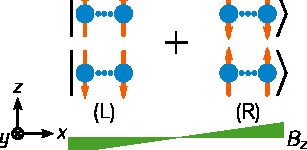
\includegraphics[scale=1.2]{img/GM_double_well.pdf}
    \caption[Best entangled state for the spatial two-ensembles]{
    (blue-circle) Atoms located at (L) or (R).
    (red-arrow) Spin state of each of the atoms.
    (green-area) Linear magnetic field $B_z$.
    Note that the $z$-axis is to represent the direction of the spins.
    On the other hand, the state is a linear superposition of the upper state and the lower state, represented by $\ket{\cdot}$ and $+$ sign.
    Note that all particles at (L) or (R) are assumed to be in the same spatial spot.}
    \label{fig:gm-double-well}
  \end{center}
\end{figure}

We compute first the $\qfif{\rho^{(\text{s})},j_z^{(n)},j_z^{(m)}}$ for $\ket{\Psi}$ as
\be
  \qfif{\ket{\Psi},j_z^{(n)},j_z^{(m)}}=\lcor
  \begin{aligned}
    & 4j^2  && \text{if } (n,m)\in\text{(L,L) or (R,R)},\\
    & {-4j^2} && \text{if } (n,m)\in\text{(L,R) or (R,L)}.
  \end{aligned}
  \right.
\ee
Now, if we separate the terms of the sum in Eq.~\eqref{eq:gm-bound-for-insensitive-and-thermal-state} into two groups, such that one of the sums is for indexes $(n,m)\in\text{(L,L) or (R,R)}$, and the other is for indexes $(n,m)\in\text{(L,R) or (R,L)}$, we can compute the bound for the best state for the two ensemble case as
\be
\begin{split}
  \varian{b_1}|_{\max} &=
  \sum_{\ver{(n,m)\in}{ \text{(L,L) or (R,R)}}} a^2 4j^2 + \sum_{\ver{(n,m)\in}{ \text{(L,R) or (R,L)}}} -a^2 (-4j^2)\\
  &= 4 a^2 N^2j^2.
\end{split}
\ee

On the other hand, if we compute now the standard deviation Eq.~\eqref{eq:gm-variance}, as we did before for the case of the chain Eq.~\eqref{eq:gm-variance-chain},
we have that for the two ensembles case $\mu=0$ and the standard deviation for the spatial state is
\be
  \sigma_{\text{te}}^2 = a^2,
  \label{eq:gm-variance-two-ensembles}
\ee
with which
\be
  \varian{b_1}_{\text{HL}}|_{\max} = 4 \sigma_{\text{te}}^2 N^2j^2.
  \label{eq:gm-hl-twoens}
\ee
For a general $\sigma^2$, the Eq.~\eqref{eq:gm-hl-twoens} can be seen as the Heisenberg limit for gradient metrology.
Note that the state is insensitive to the Homogeneous field, hence this bound is saturable by some measurement, and that the state $\ket{\Psi}$ maximizes the variance of $H_1$ for any given $\sigma^2$.
Before concluding, we want to show another more usual approach to the same problem.

Knowing that the QFI is convex in the state and considering the spatial state to be Eq.~\eqref{eq:gm-double-well-spatial-pdf}, we reduce our problem to the internal subspace in which the state that maximizes the QFI is the one that maximizes $(\Delta H_1)^2$.
In this case, taking into account the particle locations are given and that we have zero magnetic field at the origin, we obtain
\be
  H_{1,\text{eff}}^{(\text{s})} = a(\mtxid^{(\text{L})}\otimes J_{z}^{(\text{R})}-J_{z}^{(\text{L})}\otimes \mtxid^{(\text{R})}),
  \label{eq:gm-effective-hamiltonian-double-well}
\ee
where we write the effective Hamiltonian that the particles on the left and right feel.
This proves that we have used the right state, since it maximizes the variance $\varian{H_{1,\text{eff}}^{(\text{s})}}$ \cite{Landini2014}.

\subsubsubsection{States separable into $\ket{\psi}^{({\rm L})}\otimes\ket{\psi}^{({\rm R})}$}

Now that we have already introduced the reader to the case of the two ensembles, we take the opportunity to show some more important results for states of the form of $\ket{\psi}^{(\text{L})} \otimes \ket{\psi}^{(\text{R})}$.
These states can reach the Heisenberg limit, while they are easier to realize experimentally than states in which the particles on the left and particles on the right are entangled with each other.

First, we will compute the bound for states insensitive to the homogeneous field.
For such states we only have to compute the QFI for $H_{1,\text{eff}}$ Eq.~\eqref{eq:gm-effective-hamiltonian-double-well} such that
\be
  \varinv{b_1}|_{\max} = \qfif{\ket{\psi}^{(\text{L})}\otimes\ket{\psi}^{(\text{R})},a( \mtxid^{(\text{L})}\otimes J_{z}^{(\text{R})}-J_{z}^{(\text{R})}\otimes \mtxid^{(\text{L})})}= 2a^2\qfif{\ket{\Psi}^{(\text{L})},J_z^{(\text{L})}},
  \label{eq:gm-bound-insensitive-twoens-simplified}
\ee
where we used the general rule Eq.~\eqref{eq:bg-qfi-additive-for-tensor-product} and that any scalar multiplying the second argument of the QFI can be extracted outside the function squared.

Now, we analyze how the bound would look like for states sensitive to the homogeneous field.
Note that the single-point correlation function for particles at "(L)" and "(R)" is $a$ and $-a$ respectively, and the two-point correlation function is $a^2$ for both. Thus, in the case of computing the bound for the states sensitive to the homogeneous fields, we have that $F_{01}^{(\text{L})} = -F_{01}^{(\text{R})}$, which we used the superscript to indicate in this case over which subspace is computed the QFI matrix element, whereas the other two matrix elements we have to compute are equal for both subspaces "(L)" and "(R)".
The precision bound for states sensitive to the homogeneous fields is obtained as
\be
\begin{split}
\varinv{b_1} \leqslant &  F_{11}+\frac{(F_{01})^2}{F_{00}}\\
 =& F_{11}^{(\text{L})}+F_{11}^{(\text{R})} +\frac{(F_{01}^{(\text{L})}+F_{01}^{(\text{R})})^2} {F_{00}^{(\text{L})}+F_{00}^{(\text{R})}}\\
 =& 2F_{11}^{(\text{L})} +\frac{(F_{01}^{(\text{L})}-F_{01}^{(\text{L})})^2} {2F_{00}^{(\text{L})}}\\
 =& 2F_{11}^{(\text{L})}\\
 =& 2 a^2 \qfif{\rho^{(L)}, J_z^{(L)}},
\end{split}
\label{eq:gm-bound-sensitive-twoens-simplified}
\ee
where we use in the first line the identities for additions under tensor products Eqs.~\eqref{eq:bg-qfi-additive-for-tensor-product} and \eqref{eq:gm-FAB-additive-under-tensor}, and in the last line we extract the common factor $a^2$ and we use the linearity on the arguments the QFI.
Note that this is the same precision bound we will obtain for states insensitive to the homogeneous fields.
Note that this bound relates how good the state on the "(L)" or "(R)" subsystem is in sensing the homogeneous field with the precision achievable for the gradient parameter.
This is reasonable because the state in "(L)" is not interacting neither correlated with "(R)".
Hence, after the homogeneous field is estimated for "(L)" and "(R)" independently,
the gradient can also be estimated as the difference between the two estimates divided by the square distance $a^2$.

In the literature one can find several states that can be used to measure a homogeneous field, such as the GHZ states \cite{Greenberger1989}, unpolarized Dicke states, and spin-squeezed states.
Note that if $\ket{\Psi}$ is separable, then based in Eq.~\eqref{eq:bg-shot-noise-limit} and for any of the two bounds Eqs.~\eqref{eq:gm-bound-insensitive-twoens-simplified} and \eqref{eq:gm-bound-sensitive-twoens-simplified}, we have
\be
  \qfif{\ket{\Psi}_{\text{sep}}^{(\text{L})}\ket{\Psi}_{\text{sep}}^{(\text{R})},\,a(J_z^{(\text{L})} \mtxid^{(\text{R})}-\mtxid^{(\text{L})} J_z^{(\text{R})})}
  = 2a^2\qfif{\ket{\Psi}_{\text{sep}}^{(\text{L})}, J_z^{(\text{L})}}
  = 2a^24\frac{N}{2}j^2
  \leqslant 4a^2Nj^2.
  \label{eq:gm-snl-two-ensembles}
\ee
Note that each of the ensembles has half of the total particle number $N$.
Eq.~\eqref{eq:gm-snl-two-ensembles} can be seen as the shot-noise limit when two ensembles are used for gradient metrology.
In Table~\ref{tab:result-states-two-ensembles}, we summarized the precision bounds for states of type $\ket{\Psi}^{(\text{L})}\otimes \ket{\Psi}^{(\text{R})}$ for the two-ensemble case.
\begin{table}
  \begin{center}
    \begin{tabular}{|l|c|c|}
    \hline
    States in (L) and (R) & $\qfif{\rho,J_z}$ for $N/2$ & $(\Delta b_1)^{-2}\leqslant$ \\
    \hline
    $\ket{+j}_l^{\otimes N/2} \otimes \ket{+j}_l^{\otimes N/2} $ & $Nj$ & $ 2a^2Nj$ \\
    \hline
    %$ \ket{\text{SpSq}}\otimes\ket{\text{SpSq}}$ &  & \\
    %\hline
    $\ket{\ghz}\otimes\ket{\ghz}$ & $N^2/4$ & $ a^2N^2/2$\\
    \hline
    $\ket{\dicke{{N/2}}}_{x}\otimes \ket{\dicke{{N/2}}}_{x}$ & $N(N+4)/8$ & $ a^2N(N+4)/4$\\
      \hline
    $\ket{\Psi}_{\text{sep}}\otimes\ket{\Psi}_{\text{sep}}$ & $2Nj^2$  & $ 4a^2Nj^2$ \\
    \hline
    \end{tabular}
  \end{center}
\caption[Bounds on the precision for different states $\ket{\psi}^{(\text{L})}\otimes\ket{\psi}^{(\text{R})}$]{
(first column) The complete state as a tensor product of the state in (L) and the state in (R). Note that for the GHZ state and the unpolarized Dicke state, the spin is $j=\frac{1}{2}$.
The last state $\ket{\Psi}$ is the best separable state for the estimation of the homogeneous field.
Hence, the bound for $\ket{\Psi}$ coincides with the shot-noise limit for gradient metrology with two ensembles.
(second column) Precision of the estimation of the homogeneous magnetic field in one of the ensembles.
(third column) From the second column and based on Eqs.~\eqref{eq:gm-bound-insensitive-twoens-simplified} and \eqref{eq:gm-bound-sensitive-twoens-simplified}, we compute the precision for differential magnetometry for various product quantum states in two ensembles spatially separated from each other by a distance $a$.
Note that all states are sensitive to the homogeneous field so the saturability of of the bound is not ensured.
This is the reason we use "$\leqslant$" instead of "$|_{\max}$".
}
\label{tab:result-states-two-ensembles}
\end{table}

In this section we have shown to the reader how one should handle the spatial width of the system for classifying it for gradient metrology as well as a state-of-the-art system in which the Heisenberg limit is achieved.
Moreover, we have shown how to use the tools developed in the previous section to compute simple bounds.
In the next section we will focus on single cold-atom ensembles since they play an important role in quantum technology, and many groups are trying to realize them whit great success but with few theoretical support.

%%%%%%%%%%%%%%%%%%%%%%%%%%%%
\subsection{Magnetometry with a single atomic ensemble}
\label{sec:gm-single-cloud}
%%%%%%%%%%%%%%%%%%%%%%%%%%%%

In this section, we discuss magnetometry with a single
atomic ensemble in more detail.
We consider a one-dimensional ensemble of spin-$j$ atoms
placed in a one dimensional trap, which is elongated
in the  $x$-direction.
The magnetic field points in the $z$-direction,
and has a constant gradient along the $x$-direction.
The setup is depicted
in Fig.~\ref{fig:gm-single-ensemble-in-gradient}.
In the last part of this section, we calculate precision bounds for the
gradient estimation for some important multi-particle quantum states,
for instance, Dicke states or GHZ states.
Note that all these states are permutationally invariant, since we
assume that a permutationally invariant procedure prepared the states.
\begin{figure}[htp]
  \begin{center}
  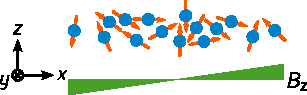
\includegraphics[scale=1.2]{img/GM_single_cloud.pdf}
  \caption[Single atomic ensemble for gradient magnetometry]{
  (blue-point) Atomic ensemble with their spins (red-arrow) pointing randomly in any direction coupled with a linear magnetic field $B_z$ (green).
  The spatial state $\rho^{(\text{x})}$ is assumed to be permutationally invariant.
  The ensemble is centered around the place at which the magnetic field is zero due to the invariance of the precision bound under translations of the system.}
  \label{fig:gm-single-ensemble-in-gradient}
  \end{center}
\end{figure}

%%%%%%%%%%%%%%%%%%%%%%%%%%%
\subsubsection{Precision bound}
%%%%%%%%%%%%%%%%%%%%%%%%%%%

In an atomic ensemble of very many atoms, typically
the atoms cannot be individually addressed.
This can be taken into account, if we consider
quantum states that are permutationally invariant.
Hence, we will consider states for which both the internal state $\rho^{(\text{s})}$ and the probability distribution function
$\prob(\bs{x})$, appearing in Eq.~(\ref{eq:gm-thermal-state}),
are permutationally invariant.
The permutational invariance of $\prob(\bs{x})$ implies that
\be
  \label{eq:pi-for-pdf}
  \prob(\bs{x})=\tfrac{1}{N!}\sum_{k}\mathcal{P}_k [\prob(\bs{x})],
\ee
where the summation is over all the possible permutations of the variables $x_n$ denoted by $\mathcal{P}_k$.

As we have shown in Section~\ref{sec:gm-cramer-rao-bounds}, the precision bound is invariant under spatial translations.
This allows us to place the "center of mass" of the system at the origin of the coordinate system.
With this simplifying assumption and based on Eqs.~\eqref{eq:gm-mean}, \eqref{eq:gm-variance} and \eqref{eq:gm-correlation}, the single-point average appearing in Eq.~\eqref{eq:gm-bound-for-sensitive-and-thermal-state} is
\be
  \int x_n \prob(\bs{x}) \, \text{d}^N\bs{x} = \int \frac{\sum_{n=1}^N x_n}{N} \prob(\bs{x}) \, \text{d}^N\bs{x} = \mu = 0,
  \label{eq:gm-single-point-average-sinens}
\ee
where we used the permutational invariance of $\prob(\bs{x})$ substitute $x_n$ by the sum appearing in Eq.~\eqref{eq:gm-mean}.
In a similar way we obtain
\be
  \int x_n x_m \prob(\bs{x}) \, \text{d}^N\bs{x} = \lcor
  \begin{aligned}
    &\sigma^2         &&\text{for } n=m,\\
    &\frac{\eta}{N-1} &&\text{for } n\neq m,
  \end{aligned}\right.
  \label{eq:gm-two-point-correlation-sinens}
\ee
where we used that the system is placed at the origin $\mu=0$.
An interesting property of the covariance of this type is that its a value is bounded from below and from above by the variance itself and the particle number $N$ in the following way,
\be
  \frac{-\sigma^2}{N-1}\leq \eta\leq \sigma^2.
\ee
Note that in the first sum in Eq.~\eqref{eq:gm-bound-for-sensitive-and-thermal-state} there are in total $N(N-1)$ terms proportional to $\eta/(N-1)$ and $N$ terms proportional to $\sigma^2$.

From the linearity in the second and third arguments of $\qfif{\rho, A, B}$ Eq.~\eqref{eq:gm-FAB} and for states insensitive to the homogeneous field, where $\qfif{\rho, J_z}=0$, we have that
\be
  \sum_{n=1}^N \qfif{\rho, j_z^{(n)}} = -\sum_{n\neq m}^N \qfif{\rho,j_z^{(n)},j_z^{(m)}}.
  \label{eq:gm-qfi-identity-insensitive}
\ee


From the definition of the QFI for states insensitive to the homogeneous field, Eq.~\eqref{eq:gm-bound-for-insensitive-and-thermal-state}, we compute the bound for single ensembles as
\be
\begin{split}
  (\Delta b_1)^{-2}|_{\max} &= \sum_{n,m}^N \int x_n x_m \prob(\bs{x}) \, \text{d}^N\bs{x} \qfif{\rho^{(\text{s})}, j_z^{(n)}, j_z^{(m)}}\\
  &=\sum_{n=1}^N \sigma^2 \qfif{\rho,j_z^{(n)}} + \sum_{n\neq m}^N \eta \qfif{\rho,j_z^{(n)},j_z^{(m)}}.
\end{split}
\ee
Together with Eq.~\eqref{eq:gm-qfi-identity-insensitive} we write the precision bound for states insensitive to the homogeneous fields as
\be
(\Delta b_1)^{-2}|_{\max} = (\sigma^2-\eta) \sum_{n=1}^{N} \qfif{\rho^{(\text{s})},j_z^{(n)}}.
\label{eq:gm-bound-insensitive-sinens}
\ee
Note that the bound in Eq.~\eqref{eq:gm-bound-insensitive-sinens}
can be saturated by an optimal measurement.
Nevertheless, it cannot surpass the
shot-noise scaling, $\sim N$, because $\qfif{\rho^{(\text{s})},j_z^{(n)}}$, the QFI for the single-particle operator $j_z^{(n)}$, cannot be larger than $j^2$.

To compute the bound for states sensitive to the homogeneous field, note that in the second term appearing in Eq.~\eqref{eq:gm-bound-for-sensitive-and-thermal-state} is proportional to the single-point average Eq.~\eqref{eq:gm-single-point-average-sinens} which was chosen to be equal to zero.
Hence, we only have to compute the first term of the Eq.~\eqref{eq:gm-bound-for-sensitive-and-thermal-state} as
\be
\begin{split}
  \varinv{b_1}\leqslant& \sum_{n,m}^N \int x_n x_m \prob(\bs{x}) \, \text{d}^N\bs{x} \qfif{\rho^{(\text{s})}, j_z^{(n)}, j_z^{(m)}}\\
  =& \sum_{n=1}^N \sigma^2 \qfif{\rho,j_z^{(n)}} + \sum_{n\neq m}^N \eta \qfif{\rho,j_z^{(n)},j_z^{(m)}}\\
  =&(\sigma^2- \eta)\sum_{n=1}^N  \qfif{\rho,j_z^{(n)}} + \eta\sum_{n, m}^N  \qfif{\rho,j_z^{(n)},j_z^{(m)}},
\end{split}
\ee
where in the second line we compute the diagonal and the off-diagonal terms of the sum separately and in the last line we add $\eta\sum_{n=1}^N \qfif{\rho,j_z^{(n)}}$ to the last term and subtract it from the first term to make the expression more similar to Eq.~\eqref{eq:gm-bound-insensitive-sinens}.

Hence, for states sensitive to homogeneous fields,
the precision of estimating the gradient is bounded from above as
\be
\label{eq:gm-bound-sensitive-sinens}
\varinv{b_1} \leqslant (\sigma^2-\eta) \sum_{n=1}^N \qfif{\rho^{(\text{s})},j_z^{(n)}} + \eta \qfif{\rho^{(\text{s})},J_z}.
\ee
The second term on the right-hand side of Eq.~\eqref{eq:gm-bound-sensitive-sinens} is new in the sense that it did not appear in the bound for states insensitive to homogeneous fields.
Note that the bound in Eq.~(\ref{eq:gm-bound-sensitive-sinens}) is not necessarily saturable if the optimal measurements to estimate the gradient parameter and the homogeneous parameter do not commute with each other.
Note also that even if the first term cannot overcome the shot-noise scaling, in the second term the covariance is multiplied by QFI for estimating the homogeneous field and therefore this concrete term can make the bound, for extremely correlated particle positions, to scale as Heisenberg scaling.

%%%%%%%%%%%%%%%%%%%%%%%
\subsubsection{Precision bounds for different spin-states}
%%%%%%%%%%%%%%%%%%%%%%%

In this section, we present the precision limits for different classes of important quantum states such as the totally polarized state, the state having the largest precision among separable states, or the singlet state.
We will calculate the precision bounds presented before, Eqs.~\eqref{eq:gm-bound-insensitive-sinens} and \eqref{eq:gm-bound-sensitive-sinens}, for these systems.
We show first the results for singlets that are insensitive to homogeneous
fields.
In this case, the bounds can be achieved by choosing
the appropriate magnitude to measure.
The rest of the results are for states sensitive to homogeneous
fields which in general are not necessarily achievable bounds.

Before going into the details of our computations we present a summary of the results obtained in this section.
The summary for different states can be found in the Table~\ref{tab:compare all the states}.
\begin{table}
  \begin{center}
  \begin{tabular}{|l|c|}
    \hline
    States & $\varinv{b_1}$ \\
    \hline
    permutationally invariant singlet states & $ |_{\max} = (\sigma^2-\eta) \frac{4Nj(j+1)}{3}$ \\
    \hline
    $\ket{+j}_{y}^{\otimes N}$ & $\leqslant \sigma^2 2Nj$ \\
    \hline
    Best separable state $\ket{\Psi}$ & $\leqslant \sigma^2 4N j^2$ \\
    \hline
    $\ket{\dicke{N}}_{z}$ & $ |_{\max}=(\sigma^2-\eta) N$\\
    \hline
    $\ket{\dicke{N}}_{x}$ & $ \leqslant (\sigma^2 -\eta) N + \eta \frac{N(N+2)}{2}$ \\
    \hline
    $\ket{\ghz}$ & $\leqslant (\sigma^2 - \eta) N  + \eta N^2$ \\
    \hline
  \end{tabular}
  \end{center}
\caption[Bounds on the precision for different states for a single atomic ensemble.]{
Precision bounds for  differential magnetometry for various quantum states.
For the definition of the states, see the text.
If the bound are proved to be saturable then
the "$|_{\max}=$" subscript is used instead of an inequality.}
\label{tab:compare all the states}
\end{table}

%%%%%%%%%%%%%%%%%%%%%%%
\subsubsubsection{Permutationally invariant singlet states}
%%%%%%%%%%%%%%%%%%%%%%%

We consider now the singlet state, which is invariant under the influence
of a homogeneous field along any direction.
So, we have to compute the formula for the bound of the precision Eq.~(\ref{eq:gm-bound-insensitive-sinens}).
A pure singlet state is an eigenstate of the collective $J_z$ and $J^2$
operators, with an eigenvalue zero in both cases.
There are many different singlet states for an ensemble of $N$
spin-$j$ particles, which some of them are permutationally invariant.
Surprisingly the precision bound we compute is the same
for any permutationally invariant singlet.
Atomic ensembles in a singlet state have been experimentally
created with cold gases \cite{Toth2010, Behbood2014}.

In an $N$-particle system, there are several singlets pairwise orthogonal to each other.
The number of such singlets, $D_0$, depends on the particle spin $j$ and the number of particles $N$.

The most general singlet state can be written in the total angular momentum basis, using $D$ to label the degenerate states, see Appendix~\ref{app:angular-subspaces}.
In its eigenbasis the singlet is written as
\be
\rho^{(\text{s})}=\sum_{D=1}^{D_0}\lambda_D\ketbra{0,0,D}{0,0,D},
\label{eq:gm-general-singlet}
\ee
where $\sum_D \lambda_D=1$.
In its complete form the eigenvalues of the spin density matrix are $\lambda_{J,M_z,D}=\delta_{0,J}\lambda_D$.

Looking at Eq.~\eqref{eq:gm-bound-insensitive-sinens},
we must compute the QFI for the one-particle operator $j_z^{(n)}$ in order to compute the precision bound for permutationally invariant singlet states.
For that purpose we use the fact that when $j_z^{(n)}$ acts on a singlet state, it produces a state outside of the singlet subspace.
This can be proved by noting that
\be
  e^{i \pi J_x} j_z^{(n)} e^{-i \pi J_x}=-j_z^{(n)}
\ee
and that $e^{-i\pi J_x} \ket{0,0,D} = \ket{0,0,D}$
holds for any pure singlet state.
Hence, we can arbitrarily flip the sign of $j_z^{(n)}$ so
\be
  \bra{0,0,D}{j_z^{(n)}}\ket{0,0,D'}
  =-\bra{0,0,D}{j_z^{(n)}}\ket{0,0,D'},
\ee
which implies
\be
  \bra{0,0,D}{j_z^{(n)}}\ket{0,0,D'}=0,
  \label{eq:gm-expectation-jzn-for-singlets}
\ee
for any pair of pure singlet singlet states.

In order to compute the QFI for the singlet state we use
Eq.~\eqref{eq:gm-FAB-rewrite-with-trace}.
Hence, we can write the following for the second term on Eq.~(\ref{eq:gm-FAB-rewrite-with-trace}),
\be
  8\sum_{D,D'}
  \tfrac{\lambda_D\lambda_{D'}}
  {\lambda_D+\lambda_{D'}}
  |\bra{0,0,D}{j_z^{(n)}}\ket{0,0,D'}|^2=0.
\ee
It follows that the QFI of $j_z^{(n)}$ for any singlet is indeed simply
\be
  \label{eq:gm-qfi-as-trace-singlet}
  \qfif{\rho^{(\text{s})}, j_z^{(n)}}
  =4\tr({\rho^{(\text{s})} (j_z^{(n)})^2}).
\ee

Finally, we must compute the expectation value of the operator $(j_z^{(n)})^2$.
For that we have that
\be
  \tr(\rho^{(\text{s})}(j_k^{(n)})^2)
  =\tr(\rho^{(\text{s})}(j_l^{(n)})^2),
\ee
for any pair $k,l\in x,y,z$ due to the rotational invariance of the singlet, i.e, all the singlets remain invariant under a $SU(2)$ transformation of the kind $U=e^{i\phi J_{\bs{n}}}$, where $\bs{n}$ is an unitary vector belonging to the positional space.
Then we can write that
\be
\expect{(j_x^{(n)})^2+(j_y^{(n)})^2+(j_z^{(n)})^2}=j(j+1),
\ee
for any state, since it represents the spin number of the particle, which is fixed.
Hence, the expectation value of $(j_z^{(n)})^2$ on the singlet is
\be
  \label{eq:gm-expectation-jzn2-for-singlets}
  \tr(\rho^{(\text{s})}(j_z^{(n)})^2)=\frac{j(j+1)}{3},
\ee
for all the singlets.
Inserting this into Eq.~\eqref{eq:gm-qfi-as-trace-singlet} and using Eq.~\eqref{eq:gm-bound-insensitive-sinens}, we
obtain
\be
  \label{eq:gm-precision-singlet}
  \varinv{b_1}_{\text{s}}|_{\max} =\lpar\sigma^2-\eta\rpar \frac{4Nj(j+1)}{3}.
\ee

To conclude, singlet states are insensitive to homogeneous magnetic fields, hence determining the gradient leads to a single-parameter estimation problem.
This implies that there is an optimal operator that saturates the precision bound given by Eq.~\eqref{eq:gm-precision-singlet}.
However, it is usually very hard to find this optimal measurement,
although a formal procedure for this exists \cite{Paris2009, Ragy2016}.
In Ref. \cite{Urizar-Lanz2013}, a particular set-up for determining the magnetic gradient with permutationally invariant singlet states was suggested by the measurement of the $J_x^2$ collective operator.
For this scenario the precision is given by the error propagation formula as
\be
\label{eq:gm- Jx2_acc}
(\Delta b_1)^{-2}
= \frac{|\partial_{b_1}\expect{J_x^2}|^2}{\expect{J_x^4}-\expect{J_x^2}^2}.
\ee

%%%%%%%%%%%%%%%%%%%%%%%
\subsubsubsection{Totally polarized state}
%%%%%%%%%%%%%%%%%%%%%%%

The totally polarized state can easily be prepared experimentally.
It has already been used for gradient magnetometry with a single atomic ensemble \cite{Koschorreck2011,Vengalattore2007}.
For the gradient measurement as for the measurement of the homogeneous field, the polarization must be perpendicular to the field we would like to measure in order to take advantage of the interaction between the particles and the field.
Here we chose as before the totally polarized state along the $y$-axis which is written as $\ket{j}_y^{\otimes N}$.
Note that this state is sensitive to the homogeneous field, hence, we must use the Eq.~(\ref{eq:gm-bound-sensitive-sinens}) to compute the bound.

For the pure states we have that $\qfif{\ket{\psi}, A} = 4(\Delta A)^2$.
Together with,
$(\Delta j_z^{(n)})^2=j/2$ and $(\Delta J_z)^2=Nj/2$, when the polarization is
perpendicular to the $z$-direction, the precision will be computed straightforward from Eq.~\eqref{eq:gm-bound-sensitive-sinens}.

Therefore, the Cram\'er-Rao bound fixes the highest value for the precision
of the totally polarized state as
\be
  \varinv{b_1}_{\text{TP}}\leqslant \sigma^2 2Nj  .
\ee
Note that the precision bound for the totally polarized state
is smaller than that of the optimal separable state we present later on.
We can see clearly that the precision scales as $\mathcal{O}(N)$.

Let us now see, which quantities have to be measured to estimate the field gradient with a totally polarized state.
The homogeneous field rotates all spins by the same angle, while the gradient rotates the spin at different positions by a different angle.
Due to that, the homogeneous field rotates the collective spin, but does not change its absolute value.
On the other hand, the field gradient decreases the absolute value of the spin, since it has been prepared to be maximal, which has been used in Ref.~\cite{Behbood2013} for gradient magnetometry, see Figure~\ref{fig:ionchain-evolution}.

%%%%%%%%%%%%%%%%%%%%%%%
\subsubsubsection{The best separable state}
%%%%%%%%%%%%%%%%%%%%%%%

We will now turn our attention to the precision bound for all separable spin states.
It is useful to obtain this value so we have a direct comparison on what is the best classically achievable precision.
It will turn out that for $j>\frac{1}{2},$ it is possible
to achieve a precision higher than with the fully polarized state.
One has to take into account that if the state is insensitive to the homogeneous field the bound can be saturated for sure, and if the state is sensitive to homogeneous fields, it would depend on the measurements compatibility and on the system as we discussed before.
From another point of view and instead of using the Eqs.~\eqref{eq:gm-bound-insensitive-sinens} and \eqref{eq:gm-bound-sensitive-sinens}, what we have is that the bound is the same $\qfif{\rho, H_1}$ for both cases.
Note that we can place the system at the point in which the magnetic field is zero without changing the result.
Thus, it is easy to argue that the precision bound itself is a convex function on the states.
Moreover, it is also a convex function of the states when the external state $\rho^{(\text{x})}$ is fixed and only the internal $\rho^{(\text{s})}$ is considered.

In the single ensemble configuration, Eq.~\eqref{eq:gm-f11-thermal} must be computed only, where the two-point correlation function returns $\sigma^2$ or $\eta$ based on Eq.~\eqref{eq:gm-two-point-correlation-sinens}.
On the other hand, for pure states we have that $\qfif{\rho^{(\text{s})}, j_z^{(n)}, j_z^{(m)}}$ is four times the correlation $\expect{j_z^{(n)}j_z^{(m)}}-\expect{j_z^{(n)}}\expect{j_z^{(m)}}$.
If the state is a product state, then we have  $\expect{j_z^{(n)}j_z^{(m)}}-\expect{j_z^{(n)}}\expect{j_z^{(m)}}=0$ for all $n\neq m$.
Hence, $\eta$ does not play any role in the precision.
Finally, we have to maximize only the variance of each of the single particle operators $4(\Delta j_z^{(n)})^2$.
From the definition of the variance,
\be
  \varian{j_z^{(n)}} = \expect{(j_z^{(n)})^2}-\expect{j_z^{(n)}}^2.
\ee
Hence, We try a state that approaches to zero its polarization on the $z$-direction and maximizes \expect{(j_z^{(n)})^2}.

We have that  $\ket{\Psi}=(\ket{+j}+\ket{-j})/\sqrt{2}$ is ideal for this, for any $j$.
Hence, we write the entire internal state as $\rho^{(\text{s})} =(\ketbra{\Psi}{\Psi})^{\otimes N}$.
This state gives $(\Delta j_z^{(n)})^2=j^2$ which can be used in Eq.~\eqref{eq:gm-f11-thermal} after multiplying by four.
Note that this state is permutationally invariant, hence we have finished the search for the best separable permutationally invariant state.
Moreover, the state is sensitive to the homogeneous field.

Finally, the best achievable precision for separable states is written as
\be
  \varinv{b_1}_{\text{SNL}} \leqslant  \sigma^2 4 N j^2,
  \label{eq:gm-best_separable}
\ee
where the state itself is sensitive to homogeneous fields and the shot-noise limit is achieved.
Note that in the two ensembles case $\sigma^2_{\text{te}}=a^2$ which tells us that both bounds Eqs. \eqref{eq:gm-snl-two-ensembles} and \eqref{eq:gm-best_separable} are equal.
This bound coincides with the totally polarized state studied before when the spin number $j=\frac{1}{2}$.

In the following we try to find a better precision bound making use of the presumably better entangled states.
Note that the bound for the singlet state, even if it is entangled, is above the bound for the totally polarized state but below of the bound defined for the best separable state.
Nevertheless, when the singlet state is used the effect of the homogeneous magnetic field has not to be compensated since the state is insensitive to it and thus the bound can be saturated with an optimal estimator for the gradient field.

%%%%%%%%%%%%%%%%%%%%%%%
\subsubsubsection{The unpolarized Dicke states $\ket{\dicke{N}}_z$ and $\ket{\dicke{N}}_x$}
%%%%%%%%%%%%%%%%%%%%%%%

Unpolarized Dicke states play an important role in quantum optics and quantum information science.
The unpolarized Dicke state $\ket{\dicke{N}}_l$ with a maximal $\expect{J_x^2+J_y^2+J_z^2}=\mathcal{J}_{N/2}$, defined in Eq.~\eqref{eq:app-maximum-total-angular-momentum}, and $\langle J_l\rangle=0$ for any $l\in x,y,z$ is particularly interesting due to its entanglement properties and its metrological usefulness.
This state has been created in photonic experiments \cite{Kiesel2007,Wieczorek2009,Chiuri2012} and in cold atoms \cite{Luecke2011,Hamley2012}, while a Dicke state with $\langle J_z\rangle>0$ has been created with cold trapped ions \cite{haeffner2005}.

The Dicke state $\ket{\dicke{N}}_z$ is an eigenstate of $J_z$ so insensitive to homogeneous magnetic field pointing into the $z$-direction, thus the precision can be saturated by some measurement.
In the following, $\ket{\dicke{N}}_z$ without the subscript $z$ refers to $\ket{\dicke{N}}_z$.
On the other hand, the Dicke state $\ket{\dicke{N}}_x$ is sensitive to the homogeneous field.
Moreover it is very useful for homogeneous magnetometry as it has been shown in Ref.~\cite{Holland1993}.
Here we consider large particle numbers, to make the results simpler.

Since both Dicke states are pure, and following the procedure we used in previous sections, we have that to compute all the $\qfif{\rho^{(s)},j_z^{(n)}}=4(\expect{j_z^{(n)}j_z^{(m)}}-\expect{j_z^{(n)}}\expect{j_z^{(m)}})$ and $\qfif{\rho^{(s)},J_z}$ appearing in Eqs.~\eqref{eq:gm-bound-insensitive-sinens} and \eqref{eq:gm-bound-sensitive-sinens}.
Since both states are unpolarized and permutationally invariant, we have that $\expect{J_z}=0$ and $\expect{j_z^{(n)}}=0$ for both cases
Therefore, we only need to compute the second moments to compute the needed variances.

To distinguish between the to cases, $\ket{\dicke{N}}$ and $\ket{\dicke{N}}_x$, we will denote their expectation values by $\expect{\cdot}_{\dicke{}}$ and $\expect{\cdot}_{\dicke{},x}$, respectively.

First of all, from the definition of the Dicke states we have that
\be
  \expect{J_x^2+J_y^2+J_z^2} = \mathcal{J}_{N/2} = \frac{N}{2}\lpar\frac{N}{2}+1\rpar,
  \label{eq:gm-square-total-angular-momentum-dicke}
\ee
for both cases.
Moreover, $\expect{J_l^2}=0$ holds for $\ket{\dicke{N}}_l$.
The other two second moments of Eq.~\eqref{eq:gm-square-total-angular-momentum-dicke} are equal to the invariance of the states under rotations around the $l$-axis.
Hence, we can write that
\begin{subequations}
  \begin{align}
    \expect{J_z^2}_{\dicke{}} &= 0,\\
    \expect{J_z^2}_{\dicke{},x} &= \frac{\mathcal{J}_{N/2}}{2}.
  \end{align}
  \label{eq:gm-expect-jz2-both-dicke}
\end{subequations}
For the single spin components
\be
  \expect{(j_x^{(n)})^2+(j_y^{(n)})^2+(j_z^{(n)})^2}=\mathcal{J}_{1/2}
\ee
holds.
Invoking the rotational symmetry again and that $\expect{J_l^2}=\sum_{n,m}^N \expect{j_l^{(n)}j_l^{(m)}}$, we arrive at
\begin{subequations}
  \begin{align}
    \expect{(j_z^{(n)})^2}_{\dicke{}}   &= \frac{1}{4},\\
    \expect{(j_z^{(n)})^2}_{\dicke{},x} &= \frac{1}{4},
  \end{align}
  \label{eq:gm-expect-jzn2-both-dicke}
\end{subequations}
after solving a system of linear equations.

Substituting Eqs.~\eqref{eq:gm-expect-jz2-both-dicke} and \eqref{eq:gm-expect-jzn2-both-dicke} into Eqs.~\eqref{eq:gm-bound-insensitive-sinens} and \eqref{eq:gm-bound-sensitive-sinens}, the bounds for unpolarized Dicke states insensitive to the homogeneous field and sensitive to the homogeneous field are
\begin{subequations}
  \begin{align}
    \varinv{b_1}_{\dicke{}}|_{\max} &= (\sigma^2 -\eta)N,
    \label{eq:gm-bound-dicke-insensitive} \\
    \varinv{b_1}_{\dicke{},x} &\leqslant (\sigma^2 -\eta)N + \eta \frac{N(N+2)}{2},
    \label{eq:gm-bound-dicke-sensitive}
  \end{align}
\end{subequations}
where Eq.~\eqref{eq:gm-bound-dicke-sensitive} shows in principal a Heisenberg scaling behavior in the second term, whenever the particles are very correlated among each other in the position subspace.
This is due to the metrological enhancement for the sensing of the homogeneous field.
In the next section, we will see another example of a state useful for homogeneous field estimation that is also useful for gradient magnetometry.

%%%%%%%%%%%%%%%%%%%%%%%
\subsubsubsection{The GHZ state}
%%%%%%%%%%%%%%%%%%%%%%%

The Greenberger-Horne-Zeilinger (GHZ) state is also highly entangled and plays an important role in quantum information theory \cite{Greenberger1990}.
They have been created experimentally in photonic systems \cite{Pan2000,Yao2012,Lu2007} and trapped ions \cite{Sackett2000,Monz2011}.

We invoke the definition of the GHZ states Eq.~\eqref{eq:lt-ghz-state} as
\be
  \ket{\ghz} = \tfrac{1}{\sqrt{2}}(\ket{0\cdots0}+\ket{1\cdots1}).
  \label{eq:gm-ghz-state}
\ee
where $\ket{0}$ and $\ket{1}$ stands for particles with eigenvalue $-1/2$ and $+1/2$ respectively for the one-particle $j_z^{(n)}$ operator.
The state Eq.~\eqref{eq:gm-ghz-state} is very sensitive to the homogeneous field.

In order to calculate the bound explicitly, let us recall that for pure states the QFI is simplified to $\qfif{\rho,A}=4\varian{A}$ Eq.~\eqref{eq:bg-qfi-for-pure-states}.
Following the Eq.~\eqref{eq:gm-bound-sensitive-sinens}, for the GHZ state the expectation values of $j_z^{(n)}$ and $J_z$ are equal to zero, and $\expect{(j_z^{(n)})^2}=\frac{1}{4}$ and $\expect{J_z^2} = \frac{N^2}{4}$.
Hence, the variances of $j_z^{(n)}$ and $J_z$ can be computed.
Finally, we obtain the precision bound for gradient magnetometry for the GHZ state as
\be
\label{eq:gm-precision bound for ghz}
\varinv{b_1}_{\ghz} \leqslant (\sigma^2 - \eta) N  + \eta N^2.
\ee
This means that we can reach the Heisenberg-limit with such states, but only in
cases where $\eta$ is positive, i.e, that the particles stay spatially correlated.

Summarizing, we have shown different setups for the external state which could be used for gradient metrology.
We have have applied our methods for different spin states.
We can conclude with that some overcome the shot-noise limit, even when the spatial state is a single ensemble of atoms which opens up the possibility of ultra-precise gradient magnetometry with fewer experimental effort.
